\documentclass{article}

\usepackage{kern}

\begin{document}
    \begin{table}[h]
        \centering
        \begin{tabular}{c|l|l|r}
            \textbf{Durchgang} & $f_L$ in $\si{\hertz}$ & Signal in $\si{\micro\volt}$ & $u(U_{\textit{FID}})$ in $\si{\micro\volt}$\\
            \hline
            $1$ & $2007.33$ & $81.0178$ & $25.4626$\\
            $2$ & $2000$ & $73.6923$ & $26.0124$
        \end{tabular}
        \caption{Messwerte der Lamourfrequenz $f_L$ und die Unsicherheit der FID Amplutude $U_{\textit{FID}}$ zusammen mit dem bei $f_L$ gemessenen Signal in zwei Durchgängen.}
        \label{tab:2:Lamour_Freq}
    \end{table}
    An dieser Stelle macht es keinen Sinn, eine direkte Aussage über die Unsicherheit in $f$ zu tätigen, da diese Gerätespezifisch aufgelöst wird und unter der Fouriertransformation mit der Signalunsicherheit des FIDs zusammenhängt. Wir können hier somit lediglich auf diese durch die letzte Spalte der Tabelle \ref{tab:2:Lamour_Freq} Bezug nehmen, indem wir die Standardabweichung der FID Werte bestimmen. In den Graphen \ref{fig:2:Spectrum-1} und \ref{fig:2:Spectrum-2} sind die Peaks bei den ermittelten Lamourfrequenzen deutlich erkennbar.
    \begin{figure}[h]
        \centering
        \begin{subfigure}[b]{0.4\textwidth}
            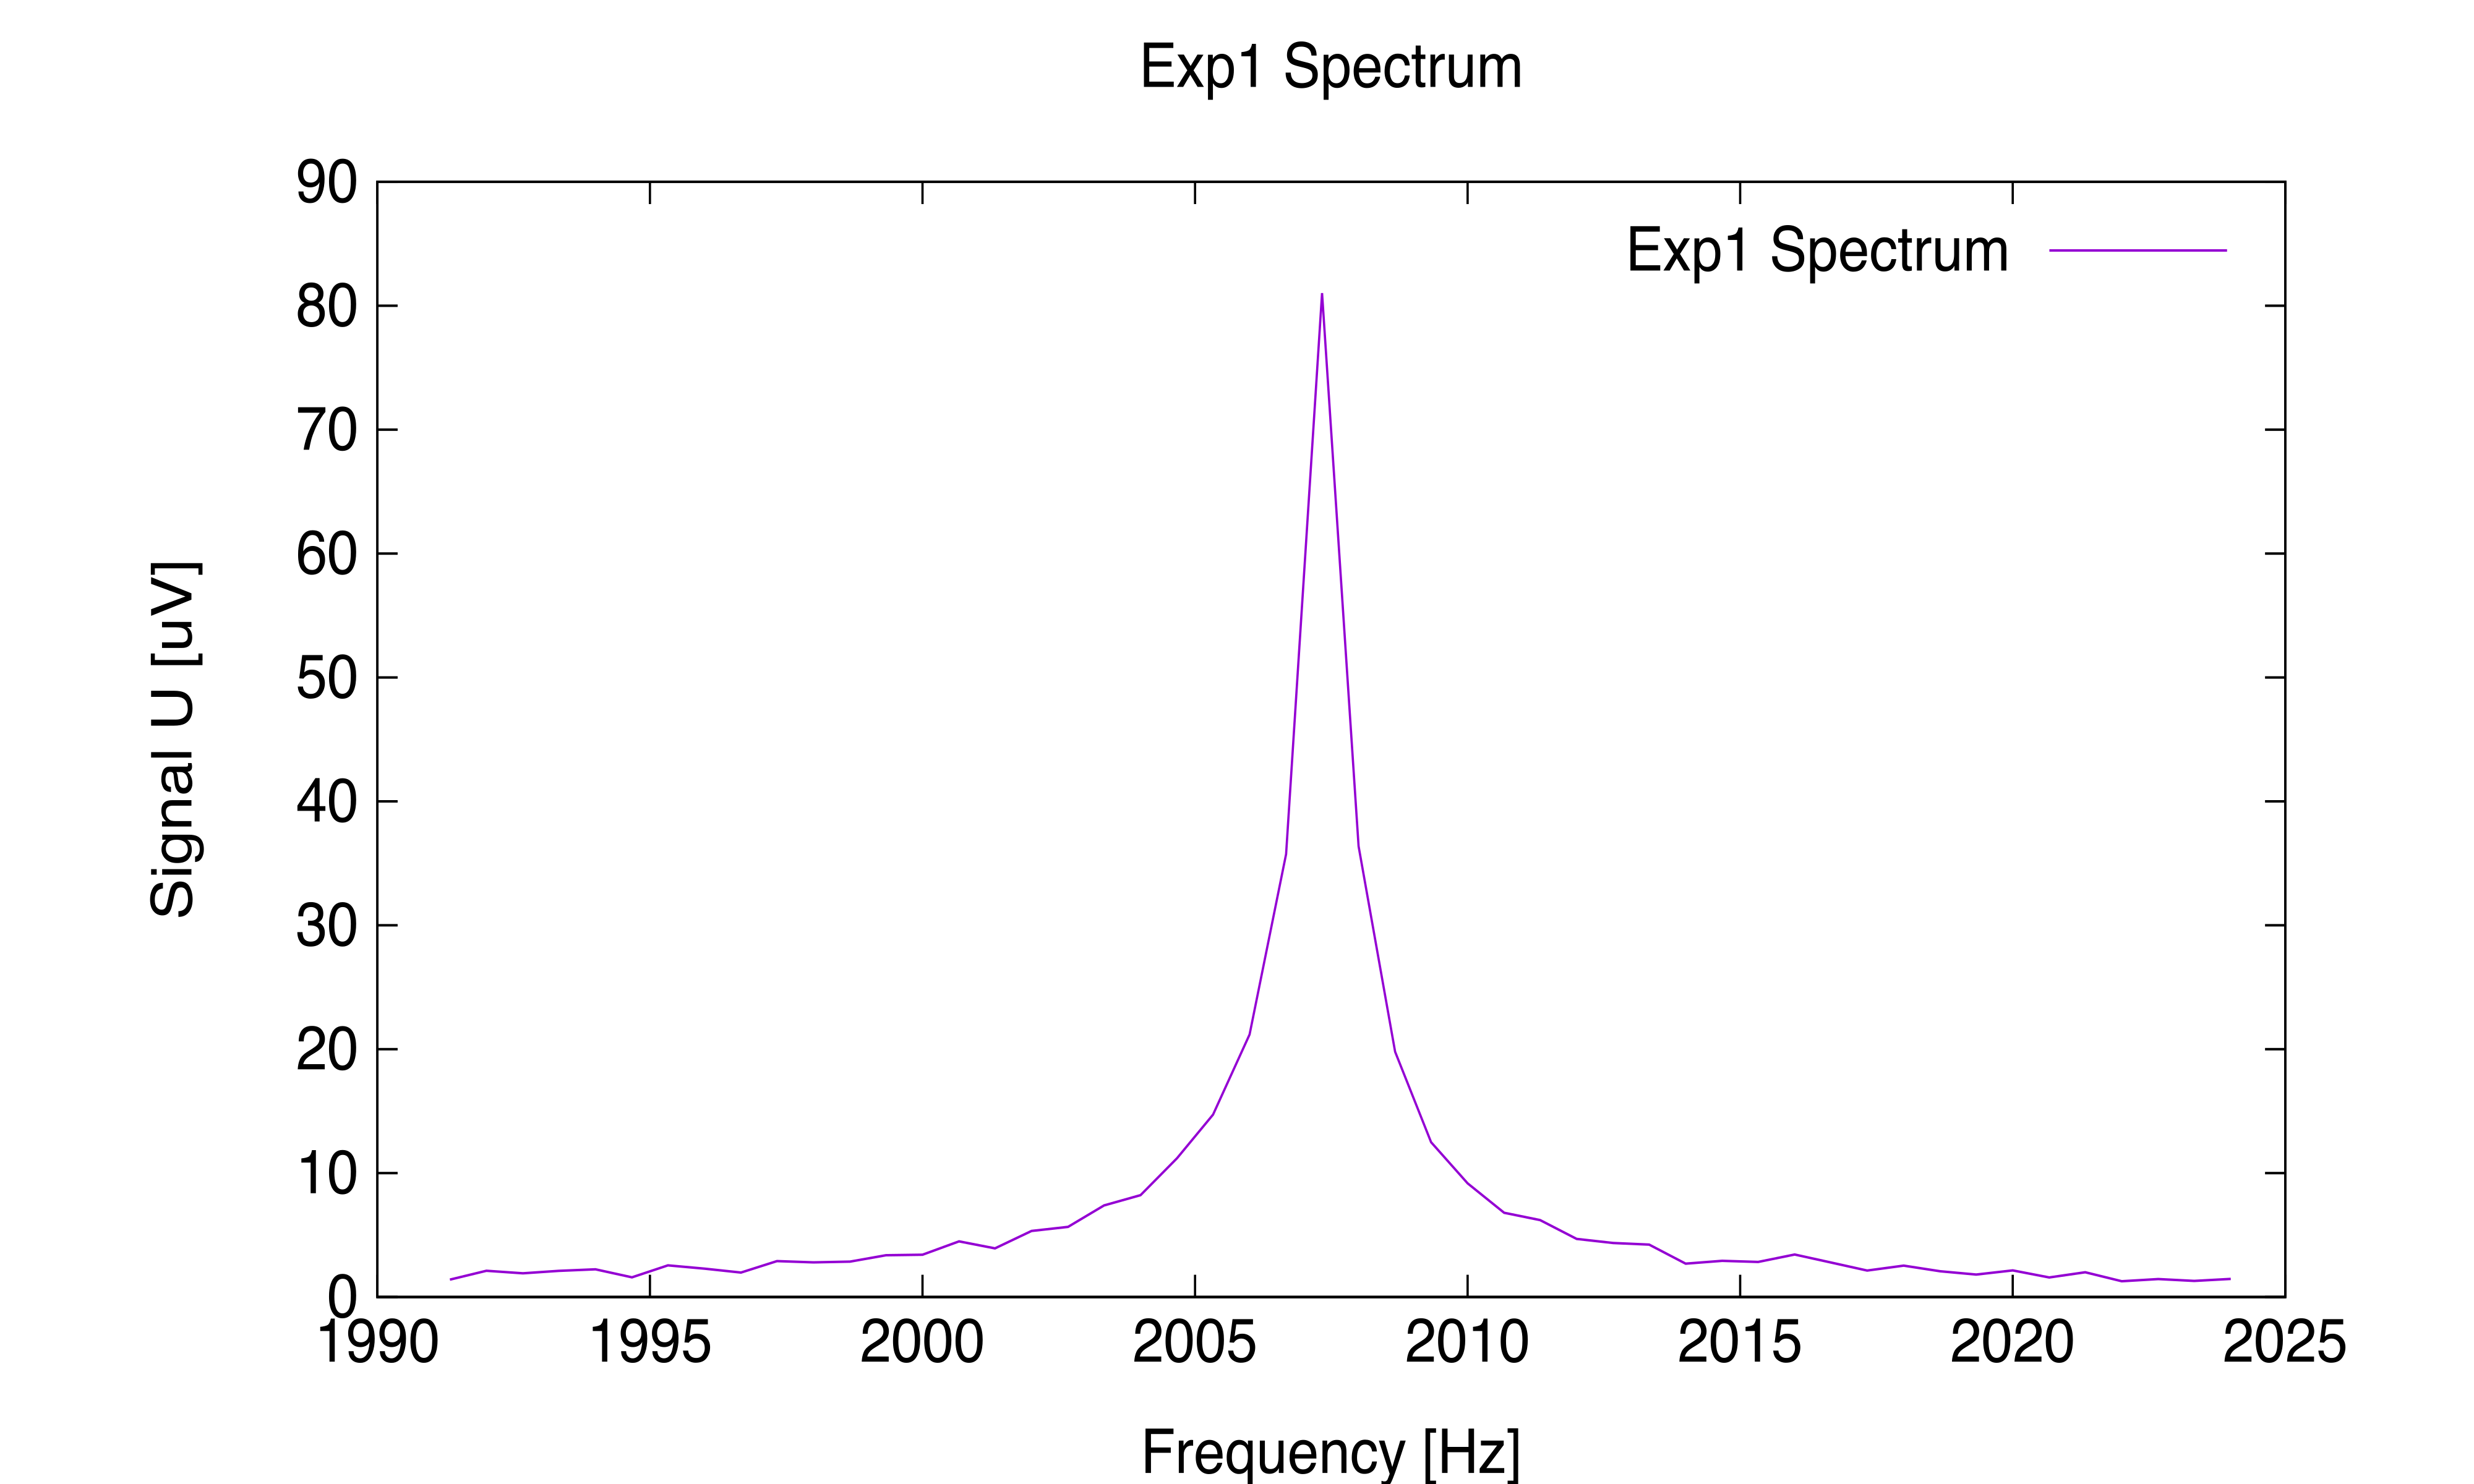
\includegraphics[width=6cm]{../Bilddateien/Exp1_Spectrum.png}
            \caption{Spektrum des FIDs mit Lamourfrequenz $f_L = \SI{2007.33}{\hertz}$.}
            \label{fig:2:Spectrum-1}
        \end{subfigure}
        \
        \begin{subfigure}[b]{0.4\textwidth}
            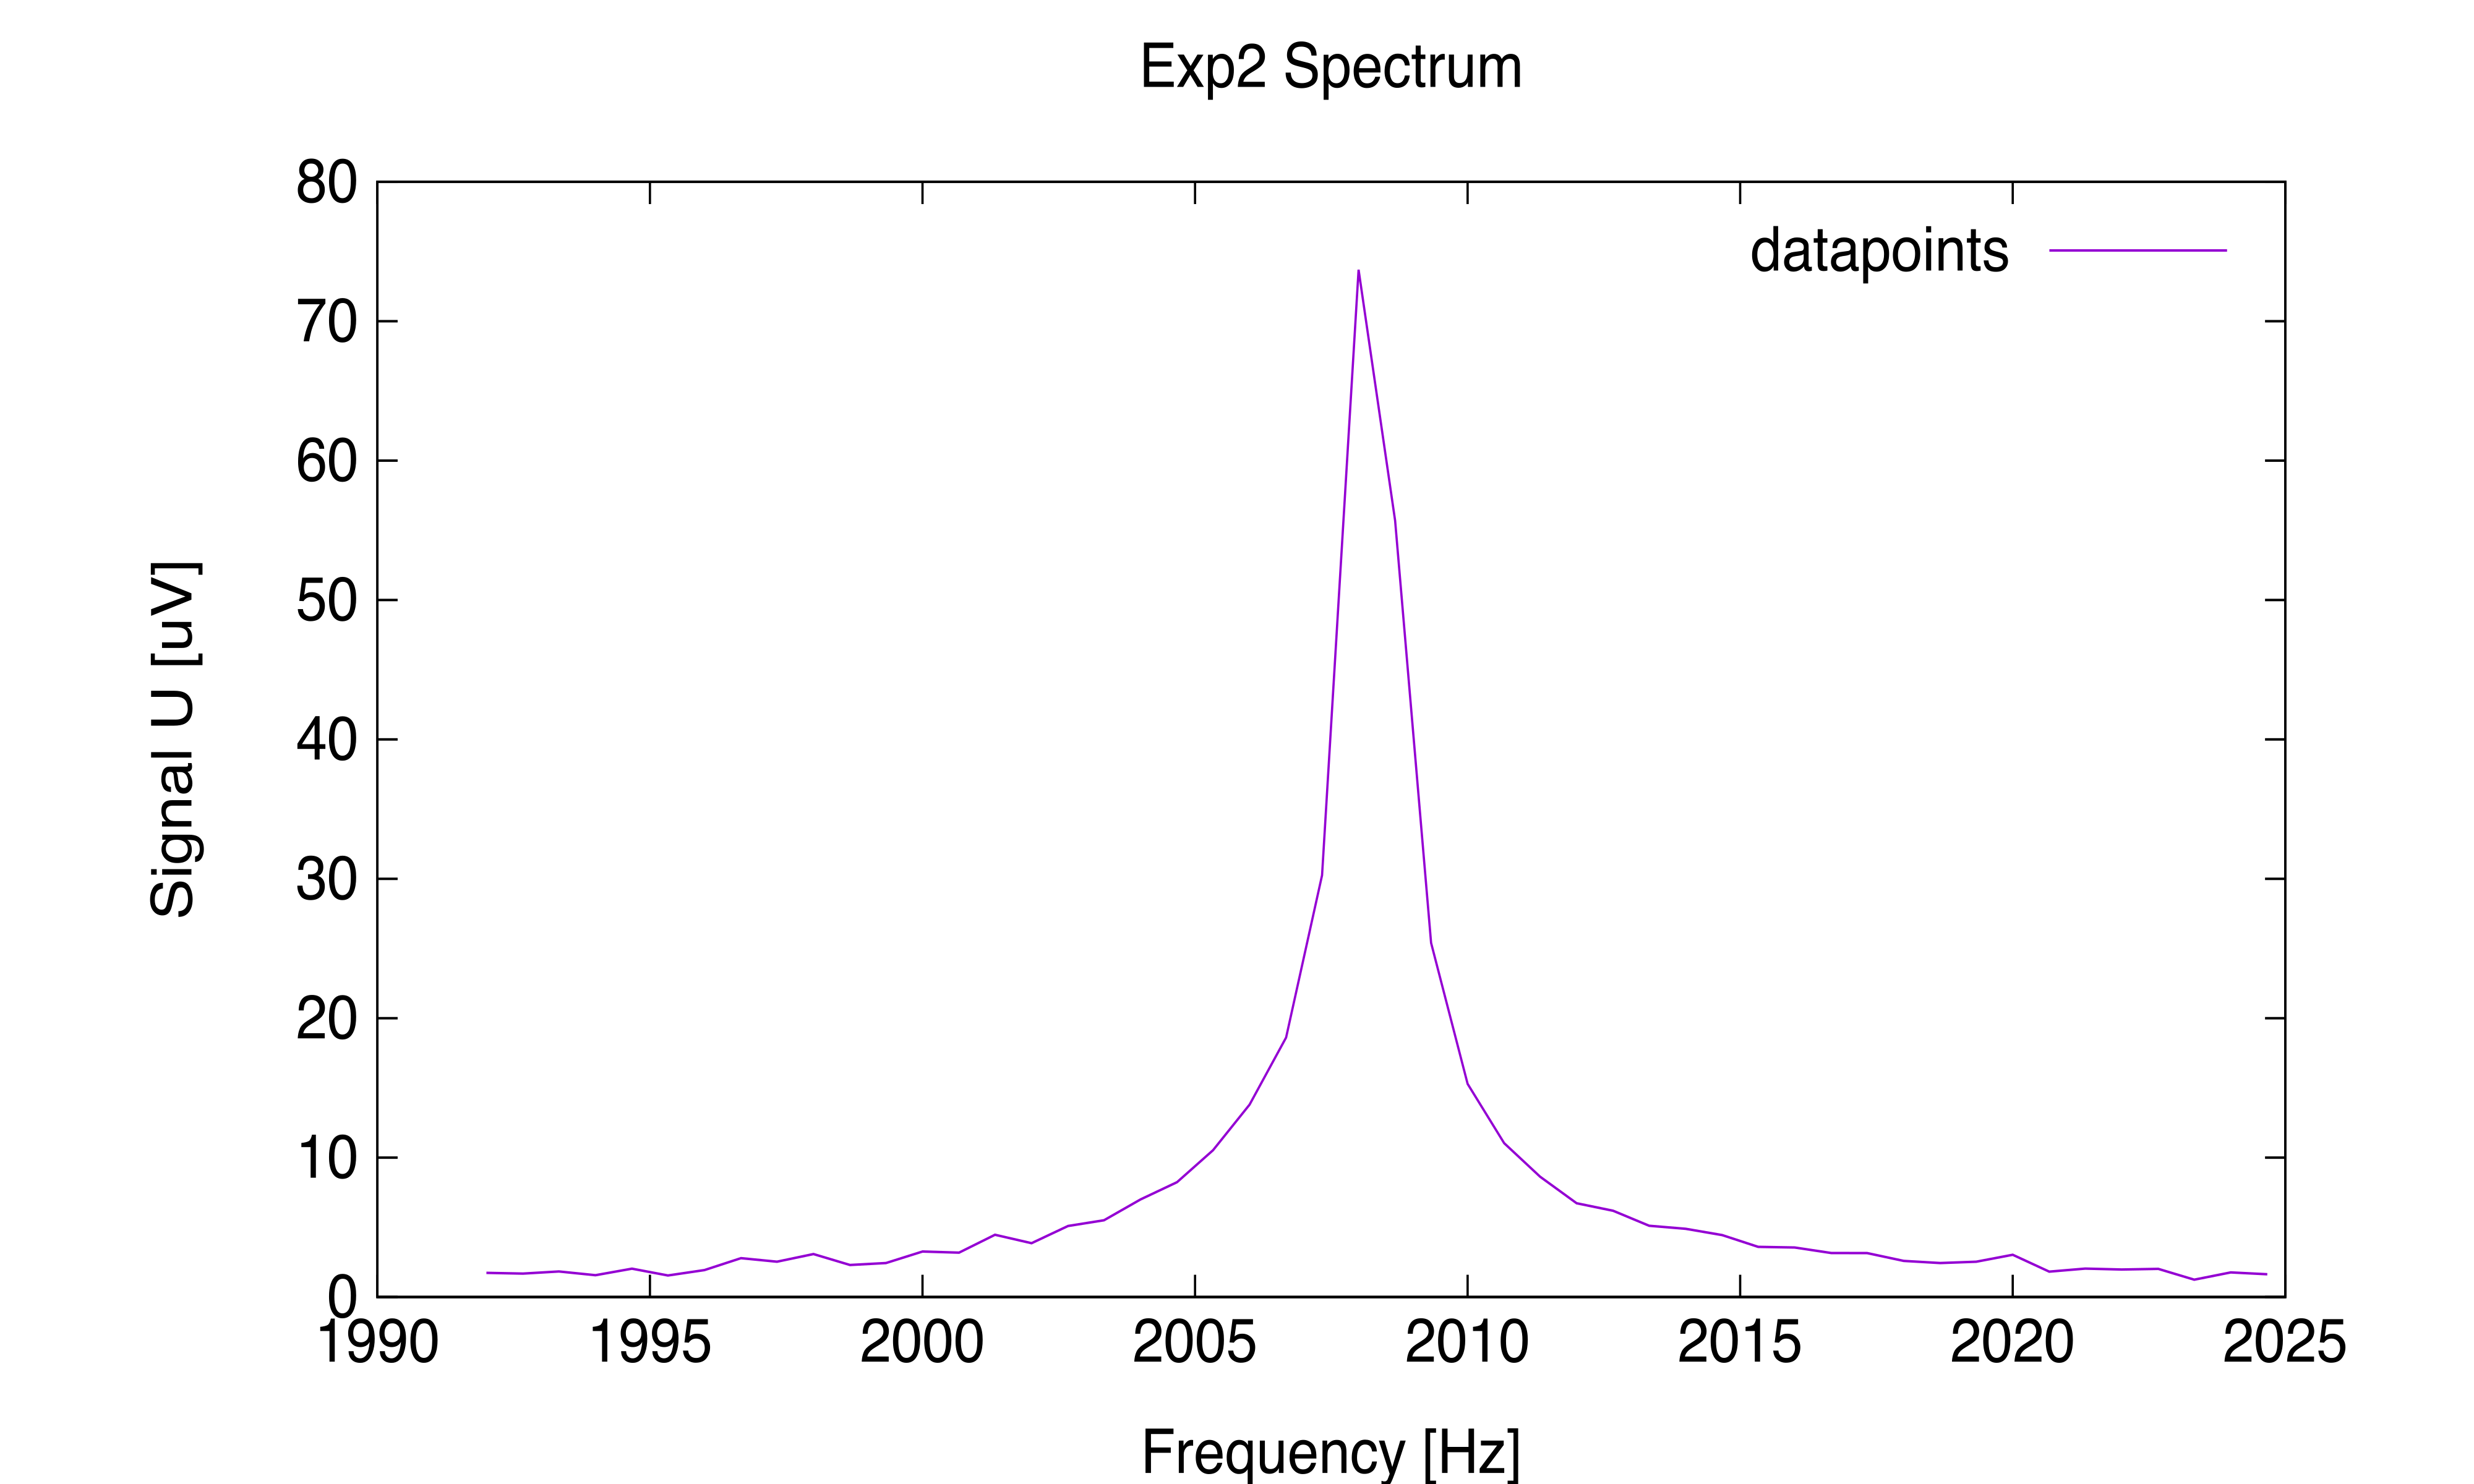
\includegraphics[width=6cm]{../Bilddateien/Exp2_Spectrum.png}
            \caption{Spektrum des FIDs mit Lamourfrequenz $f_L = \SI{2000}{\hertz}$.}
            \label{fig:2:Spectrum-2}
        \end{subfigure}
        \caption{Spektren der FIDs mit den ermittelten Lamourfrequenzen.}
    \end{figure}
\end{document}